\chapter{Design and implementation}
In this chapter we delve into the design and the implementation details of
\TOOL, the tool we built to generate SEFL models from iptables configurations
with the end goal of having them embedded in complex networks which can then be
verified using SymNet.

We begin with a high-level outline of the computation steps that take place
between dumping iptables configurations to returning a model as expected by
SymNet.  Following that, we take each of those steps separately and discuss the
most important aspects of their implementation details.


\section{Design overview}

\TOOL is essentially a compiler: its input is a file that aggregates per-table
rules dumped by the \emph{iptables} command line tool, and it outputs two Map
data structures expected by SymNet, one for port connections and the other for
port instructions (\labelindexref{Section}{sec:first-steps}).  Alternatively,
it can return a Scala object modelling the whole device if integration with
other network components is desired.

Driven by this observation, we designed \TOOL to mimic the internal
structure of a compiler too; it features three separate, well-defined phases:
\begin{itemize}
  \item \textbf{Parsing}. The input file is read and an in-memory Abstract
    Syntax Tree (AST)\abbrev{AST}{Abstract Syntax Tree} is built.  It
    materializes the hierarchy shown in
    \labelindexref{Figure}{fig:iptables-hierarchy}.
  \item \textbf{Validation}.  This step resembles \emph{semantic analysis} in
    usual compilers and its purpose is twofold:
    \begin{enumerate*}[i)]
      \item ensures that the configurations conform to the official
        specifications, and
      \item augments the AST with additional semantic information that either
        could not be gathered during parsing or it yields a more robust design
        to do it now.
    \end{enumerate*}
  \item \textbf{Code generation}. This phase is essential in any compiler and
    ours is no exception: based on the now validated in-memory AST we generate
    SEFL code for every rule as a two step process: first generate the
    constraints that correspond to rule's matches, and then
    generate the code to follow its target.

    In addition to that, we also consider as part of this step putting all
    things together according to the model template devised in the previous
    chapter (\labelindexref{Figure}{fig:iptables-2} and
    \labelindexref{Figure}{fig:chain-internal}).  We call it a \emph{template}
    because it is only a model once we fill it with real rules.  In fact, this
    step is similar to the \emph{backend} component in a compiler that is tied
    to a concrete machine architecture instead of an abstract one.  Until this
    step, the AST is a simplified and better organized view of the input rules
    but it still abstract enough to target various table/chain structures.
\end{itemize}

\begin{figure}[h]
  \centering
  \captionsetup{justification=centering}
  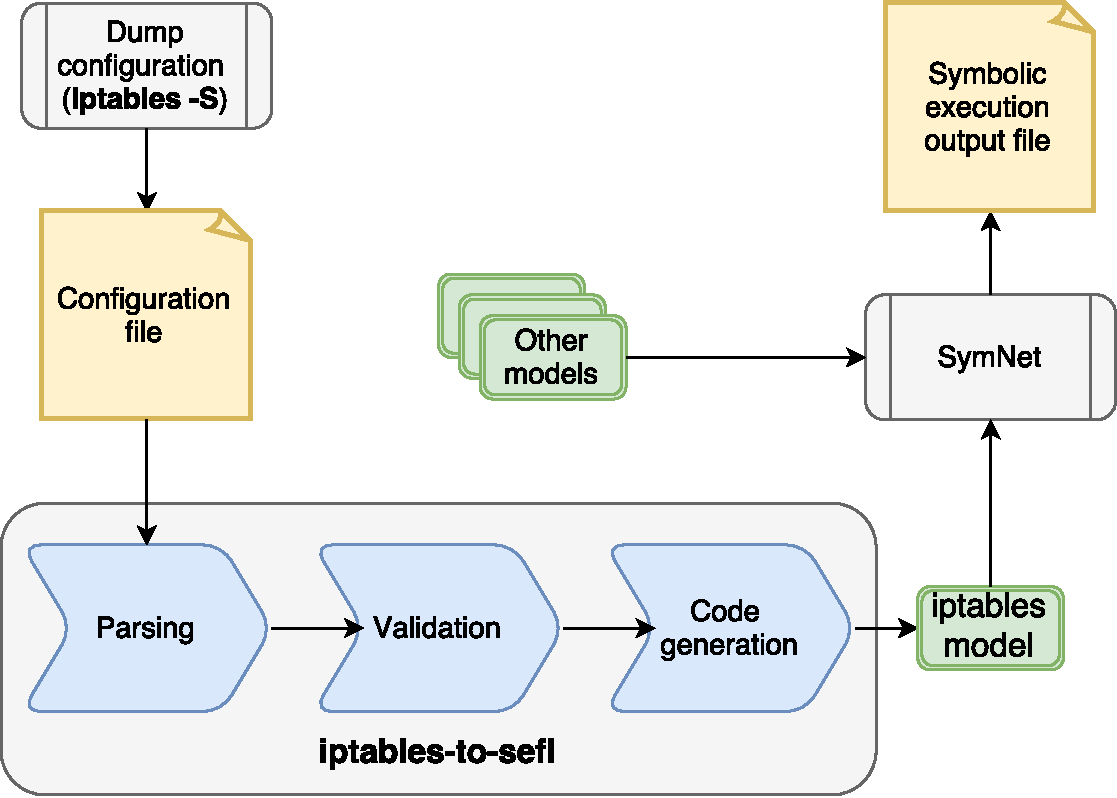
\includegraphics[scale=0.5]{src/img/high-level-design}
  \caption{High-level design of \TOOL.}
  \label{fig:high-level-design}
\end{figure}

Feeding the resulted model to SEFL, possibly alongside models of other network
elements, can be regarded as a fourth step and is included in
\labelindexref{Figure}{fig:high-level-design} which is a high-level overview of
how our tool fits in the big picture of network verification using SymNet.
Similarly, dumping the configs can be considered step zero.

Nodes in AST are called \textbf{IptElement}s.  The class hierarchy that makes
the core of \TOOL is presented in \labelindexref{Figure}{fig:ipt-hierarchy}.
It is a proper use of the composite design pattern in which multiple classes
are both \emph{components} and \emph{composites} at the same time (e.g.
\emph{Chain}, \emph{Rule}, \emph{NegatedMatch}).  ASTs follow the aggregation
relationships.  As with code generation, the only (concrete) types that can
change are the leaves: the matches and the targets that make up the rules.

In addition to the AST types that are used throughout all three computation
phases of our tool, it is worth introducing the class hierarchy behind our
model template too.  It is designed to clearly separate each component (i.e.
\emph{virtual device}) that we identified in the previous chapter and to make
their interconnection as smooth as possible. They are described in more detail
in \labelindexref{Section}{sec:codegen}, but the important thing to notice is
that it \emph{inherits} the composite pattern approach from our core AST
hierarchy.

\clearpage
\begin{figure}[h]
  \centering
  % \captionsetup{justification=centering}

  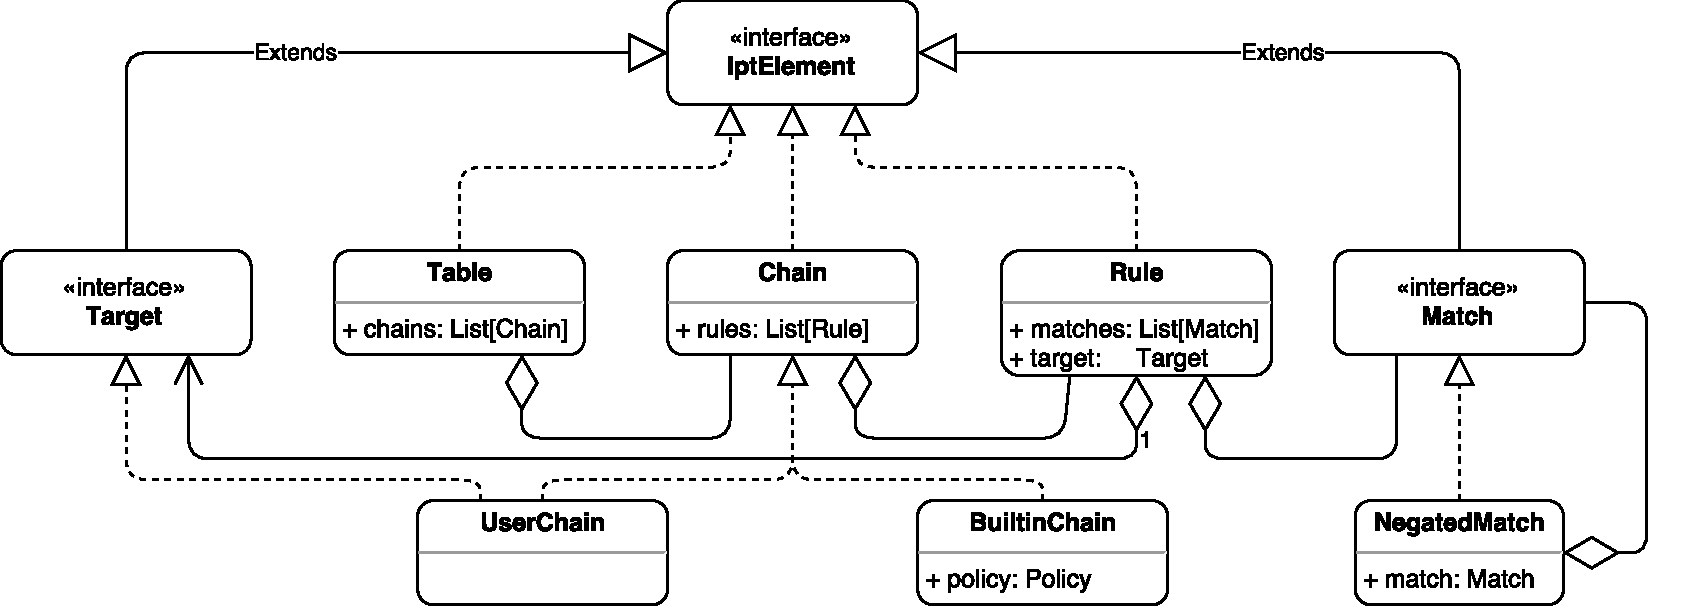
\includegraphics[scale=0.5]{src/img/ipt-hierarchy}
  \caption[The core class hierarchy in \TOOL.]{The core class hierarchy in
  \TOOL.  Interfaces \emph{Target} and \emph{Match} are the ones that must be
  subclassed when adding extensions.  It is also indicated that a
  \emph{UserChain} can be jumped to as it implements the \emph{Target}
  interface.  The \textbf{NegatedMatch} class is a utility class to
  conveniently negate another \emph{Match} instance.}
  \label{fig:ipt-hierarchy}

  \vspace*{\floatsep} % https://tex.stackexchange.com/q/26521/5764

  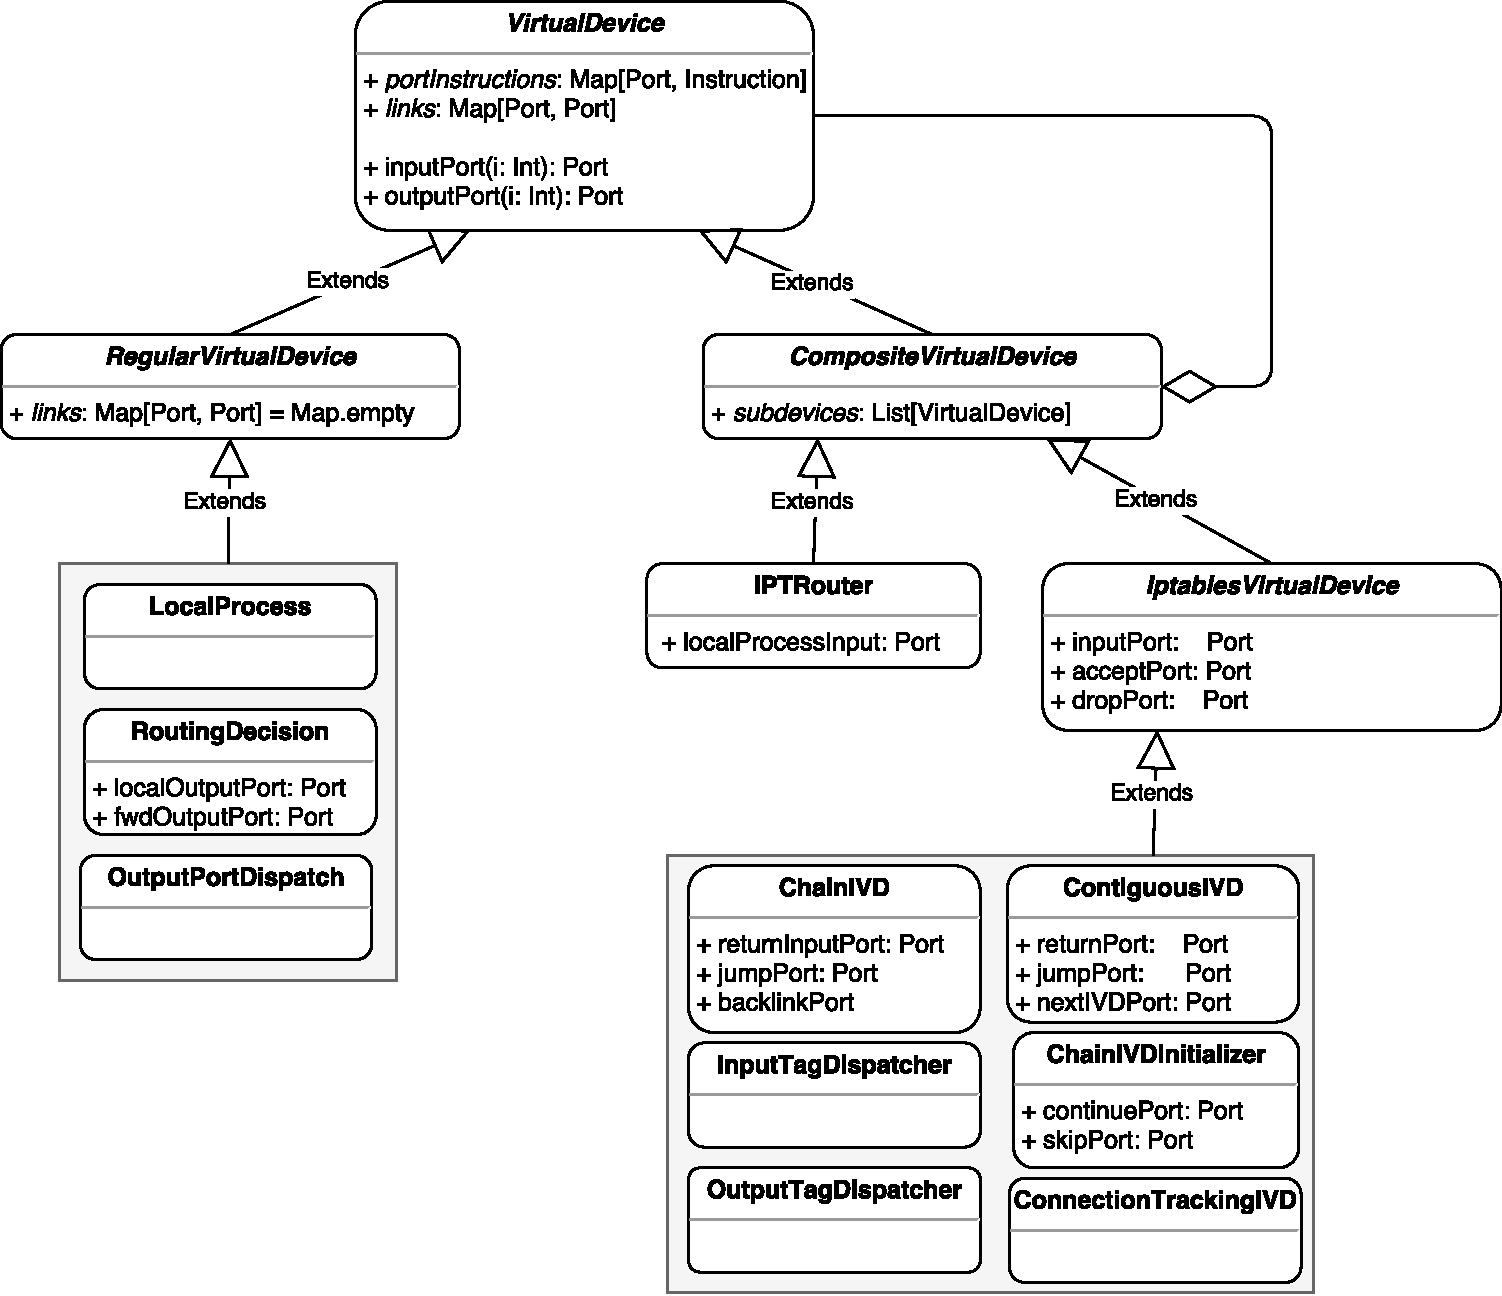
\includegraphics[scale=0.55]{src/img/virtdev-hierarchy}
  \caption[The class hierarchy of the model template part in \TOOL.]{The class
  hierarchy of the model template part in \TOOL. Besides the abstract base
  class \emph{VirtualDevice}, there are three other classes designed for
  components with certain expectations: \emph{RegularVirtualDevice} for
  self-contained ones, \emph{CompositeVirtualDevices} for components that might
  built upon some other ones, and \emph{IptablesVirtualDevice} for components
  that implement \emph{"iptables"} logic: receive packets, traverse list of
  rules and apply target, which might result in an \emph{accept} or a
  \emph{drop}.}
  \label{fig:virtdev-hierarchy}
\end{figure}
\clearpage

On top of the compiler-like internal structure, \TOOL features an
\textbf{extension-oriented design} that aims to ease as much as possible the
addition of new extensions. Since iptables supports over 100 official match and
target extensions, it is unrealistic to cover all of them upfront, in a
inextensible, monolithic design.  Even if we could, that is still not
advisable, as it is error prone and hard to debug or refactor.  To add to that,
netfilter itself is built around the idea of seamless extensibility.
Therefore, while it does not happen to often, new, fresh extensions can be
added anytime.

The building blocks of this design are the interfaces \emph{Target} and
\emph{Match} (pedantically, Scala traits), on one hand, and a generic rule
parser that can be \textbf{injected} user-defined parsers for newly added
targets and matches, on the other hand.  They are applied in the order given as
part of the \emph{ParsingContext} object.  This object gets passed and updated
during parsing and is further discussed in the section dedicated to the parsing
phase below.


\section{Parsing}\label{sec:parsing}

Our approach to iptables configuration parsing is inspired by
\textbf{Parsec}~\cite{leijen2002parsec}, a functional, monadic parser
combinator library.  The term \emph{combinator} here refers to two different
things:
\begin{enumerate}[(i)]
  \item A function with no \emph{free variables} (i.e. self-contained, pure
    function).  It is at the core of \textbf{Combinatory logic}, the theory
    behind the design of functional programming languages.
  \item A loosely defined functional design pattern.  It is centered around the
    idea of combining other (smaller) functions to reach a more complex
    functionality.
\end{enumerate}

The parsers built using this well-studied approach have a couple of desirable
properties.  Firstly, they are able to parse certain \emph{context-sensitive
grammars} by employing an LL(*), backtracking-based approach.  Secondly, they
yield loosely coupled parse rules.  Since iptables configurations can be easily
generated by a context-free grammar, our choice is mainly motivated by the
second property, especially given the extension-oriented design that we are
trying to achieve.

\labelindexref{Listing}{lst:combinators} shows some of the basic combinators
that enable us to express increasingly complex parsers.  \emph{many} and
\emph{some} are analogous to the unary operators Kleene star and its extension,
Kleene plus, respectively: they take a parser that can parse a type \textbf{T}
and repeatedly apply it, each time consuming some portion of the input.  In the
end, they return a list of \textbf{T}s parsed.  The \emph{optional} combinator
tries to parse a type \textbf{T} and returns \hlmath{Some[T]} if it succeeds or
\hlmath{None}, otherwise.  Note that the \hlmath{for/yield} syntax is a
syntactic sugar for monadic computation which propagates error implicitly,
without obfuscating the code we write.  Also, the \hlmath{$>>=$} operator is
called \textbf{bind} and is one of the defining functions behind monads.  It
takes the input altered by a parser and feeds it to the next one.

\begin{listing}[H]
  \caption{Some of the base combinators we use to build parsers.}
  \label{lst:combinators}
  \sourcecode{scala}{src/code/combinators.scala}
\end{listing}

iptables defines a grammar only for rules because chains and tables are managed
through the command line tool.  To get everything as part of a single
configuration file, we defined a simple format for chain and table
specification, starting from (and integrating) the grammar of a rule
(\labelindexref{Listing}{lst:rule-grammar}).  To get such a configuration file
from an existing deployment we also provide a script that translates from the
raw format output by issuing \texttt{iptables -S} to our format.  The complete
grammar is shown in \labelindexref{Listing}{lst:our-grammar} below.

\begin{listing}
  \small
  \lstset{numbers=none, frame=single, basicstyle=\ttfamily,
    xleftmargin=0.15\textwidth, xrightmargin=0.15\textwidth
  }
  \begin{lstlisting}
table = <<table_name>> [chains...]
chain = <chain_name> [rules...]
rule = [matches...] [target]
match = -m match_name [per-match-options]
target = -j target_name [per-target-options]
  \end{lstlisting}
  \caption{The complete grammar of an iptables configuration file.}
  \label{lst:our-grammar}
\end{listing}

As mentioned in the previous section, the extension-based design is achieved by
passing a \textbf{ParsingContext} object to the rule parser, allowing us to
keep it (besides the table and chain parsers) unchanged irrespective of the
extensions we want to turn on.  This object contains just that: lists with
match and target extensions that should be used when trying to parse a rule.
By using the \emph{implicit parameters} Scala feature this allows us to inject
various extension configurations at run time.

In addition to that, there is one more subtlety when it comes to match
extensions: the module loading part (i.e. the flags \lstinline{-m/--match}).
One might think that providing dummy parsers to \emph{consume} this part of an
iptables rule would suffice.  However, the real reason they are used is to
create a sort of \emph{namespace} for match extension options.  This means that
different extensions could use the same option and give it a completely
different meaning.  To illustrate this, let us consider the rules from
\labelindexref{Listing}{lst:namespace-example}.  Both of them use the
\lstinline{--mark} match option, although the first one refers to a metadata
field known as \emph{ctmark} (connection tacking mark) while the second one
refers to the \emph{nfmark} field (netfilter mark).

\begin{listing}
  \lstset{numbers=none, frame=single, basicstyle=\ttfamily,
    xleftmargin=0.05\textwidth, xrightmargin=0.05\textwidth
  }
  \small
  \begin{lstlisting}
-m connmark --mark 0x0/0xffff0000 -j CONNMARK --save-mark ...
-m mark ! --mark 0x2/0xffff -j SNAT ...
  \end{lstlisting}
  \caption{Two iptables rules that highlight the extension specific option
  \emph{mark} which yields different behaviours when activated by match
  extensions \emph{connmark} and \emph{mark}.  They are taken from a real-world
  OpenStack deployment.}
  \label{lst:namespace-example}
\end{listing}

How do we support this behaviour as early as parsing time?  We introduce the
notion of \emph{match-enabled extensions}.  Thus, to correctly parse (i.e.
build a correct AST) for both rules, we change our rule parser to use a
\emph{cycle-based parsing} approach: we start with two extensions that
recognize options \lstinline{-m connmark} and \lstinline{-m mark}, and leverage
our new feature by updating the current activated extensions with the ones
enabled by the previously parsed match.  Then, the next \emph{cycle} begins.

The real code that accomplishes what we have just described is presented in
\labelindexref{Listing}{lst:rule-parser}.

\begin{listing}[H]
  \caption{The implementation of the rule parser.  It uses a helper,
  tail-recursive, accumulator-based function to represent \emph{cycles}.  Each
  recursive call might modify the \emph{ParsingContext} argument by adding new
  match extensions as dictated by the previously parsed match.  An interesting
  remark is that it is one of the few parsers we defined (including the ones
  for extensions) that exceeds 15 lines of code, which is an indication of the
  effectiveness of our parsing framework in simplifying our work.}
  \label{lst:rule-parser}
  \sourcecode{scala}{src/code/rule-parser.scala}
\end{listing}


\section{Validation}

What is validation and why is it important?  As mentioned in the first section
of this chapter, the validation step in \TOOL resembles semantic analysis in
common programming language compilers: it catches errors that escaped the
parsing phase and changes or augments the AST with information or structure
needed during code generation.  We go through each one of the use cases that
are derived from this motivation in the following paragraphs.

\paragraph{Configuration checking.}
The need to ensure that the rules we test against were valid was the first
motivation for this separate computation step in \TOOL.  Not only did it help
us to better understand the semantics of each iptables feature, but it also
boosted our productivity by avoiding endless debugging when the root problem
was an incorrectly written rule.

One might ask, if this was the only motivation behind the \emph{validation}
step, would it be reasonable to disable it once we made sure that our
implementation is \emph{correct} and the rules we feed it are taken right from
an iptables dump (which we assume is correct)?  We believe that the answer is
still \textbf{no} because knowing for sure that your implementation is correct
is a very hard problem (we should know that very well), and there is an
inherent risk to introduce bugs determined by us trying to understand an
informal specification.  Therefore, there is always a chance to find out that
our tool reports validation error on a configuration file, which would have us
investigate which misunderstanding of ours caused it.  That is particularly
likely to happen as we started with very tight conditions and have
incrementally loosen them once we found that a specific scenario \textbf{is}
allowed and adapted our code to it.

How does this step reflect in code?  The \textbf{IptElement} interface provides
the method \hlmath{validate(context: ValidationContext): Maybe[Self]} that is
implemented in subclasses.  For instance, to validate a user-chain as a target
of a rule (as depicted in \labelindexref{Figure}{fig:ipt-hierarchy}) we do the
following check: \hlmath{chain != this \&\& table.chains.contains(this)}.  It
says that a user chain we jump to
\begin{enumerate*}[(i)]
  \item has to be different than the current one (\emph{recursive jumps} are
    not allowed in iptables), and
  \item should be part of the same table as the caller chain.
\end{enumerate*}

A non-exhaustive list of other configuration checks is the following (in no
particular order):
\begin{enumerate}
  \item table name validity: only \emph{raw}, \emph{mangle}, \emph{nat},
    \emph{filter} are recognized
  \item built-in chains can appear only in certain tables (e.g. FORWARD in
    \emph{mangle} and \emph{filter})
  \item some matches and targets are only valid in certain chains and tables:
    \begin{enumerate}[(i)]
      \item target DNAT is only valid in table \emph{nat}, chains PREROUTING
        and OUTPUT
      \item target DROP is allowed only in table \emph{filter}
      \item match \lstinline{--out-interface} can be used only in chains
        FORWARD, OUTPUT and POSTROUTING
    \end{enumerate}
  \item port range validity
  \item valid protocol in match \lstinline{--protocol} (can be a number or a
    name)
\end{enumerate}

We end this section with an example of a scenario in which our validation rules
were too tight, reflecting our understanding of the official specification, and
a real-world deployment proved us wrong.  Some manual pages mention that target
ACCEPT can only appear in the \emph{filter} table.  Despite being a trustworthy
source, it turned out that it can be used in any other table for
\textbf{short-circuiting} the remaining traversal of that chain.  This is one
of the desirable situations in which all we had to do was to drop one check and
still have everything work correctly.  In other scenarios, code refactoring was
needed.

\paragraph{Forward references to user chains.}
Another problem that came out early in the development process was that a user
chain might appear as part of the input configuration file \textbf{after} a
rule that jumps to it, from a previous chain.  The problem is that both a list
of \emph{Match}es and a \emph{Target} are required in order to construct an
instance of class \emph{Rule}, but at that point in the parsing process, a
reference to the \emph{yet to be parsed} chain cannot be obtained.

The way we solved it was by creating a dummy implementation of trait
\emph{Target}, called \textbf{PlaceholderTarget}, that points to a user chain
through its name only.  Thus, later, in the \emph{validation} step, we make
sure to check that the pointed-to chain does exist and replace the placeholder
with a reference to it.

This task is performed by other compilers too, especially for programming
languages that do not impose preceding declarations for referenced names.

\paragraph{Interface name wildcards.}
Lastly, a less well known feature of iptables is that a string followed by a
plus can be used to match all interfaces that are prefixed by that string, as
part of the \lstinline{--in-interface} and {\lstinline{--out-interface}
matches.  For instance, the rule \lstinline{--out-interface eth+ -j ACCEPT} can
be used to accept all traffic that exits an Ethernet interface.

Modelling string operations in an efficient manner for symbolic execution is an
open problem.  However, we can avoid doing that by statically determining the
interfaces that start with the specified string, and modify and repeat that
rule for each one of them.  For the previous rule, if our device had
interfaces \emph{eth0}, \emph{eth1} and \emph{eth2}, among others, the chain of
rules would become:

\begin{listing}
  \lstset{numbers=none, frame=single, basicstyle=\ttfamily,
    xleftmargin=0.25\textwidth, xrightmargin=0.25\textwidth
  }
  \small
  \begin{lstlisting}
<MY_CHAIN>
  [preceding rules]
  --out-interface eth0 -j ACCEPT
  --out-interface eth1 -j ACCEPT
  --out-interface eth2 -j ACCEPT
  [succeeding rules]
  \end{lstlisting}
\end{listing}

Implementation-wise, we handle this similarly to how we handled match extension
loading to avoid name clashes between different options: we add a method to
class \emph{Rule}, \hlmath{mutate(interfaces: List[String]): List[Rule]}, that
receives a list of interface names and returns a list of generated rules.  It
is called for all rules during chain validation.

A rule that does not contain any interface match will return a list containing
just itself.  One that does will return a list as shown in the previous
example.  An interesting thing to note is that it might also return an empty
list, which means that no interface matched.  This can be seen as an
optimization.  However, we would probably be much better off check-failing on
this condition and let the network administrator know that his deployment
contains a redundant rule, which is probably not intended.


\section{Code generation}\label{sec:codegen}
\todo{by code generation we mainly refer to generating code for a rule, which
means generating code for all its matches and for its target. however, in this
section we will also go into some details about the virtual device hierarchy
featured in figure X}

\todo{then start with the usual code generation: the methods for returning the
code, etc}
\todo{SeflGenOptions trait, the method for match extensions and the one for
target extensions}

\todo{tricky stuff: mention that in one of the first versions of \TOOL, the
logic for chain traversal was as simple as mentioned in a previous section; in
Scala, it was translated to two foldr operations: one to iterate through rules
from top to bottm and the other to iterate through matches of a rule. However,
along the way certain tricky things came out: rule that need "initialization",
rules that do not end the traversal of that chain}

\todo{then some details about this virtdev implementation}
\todo{maybe mention that classes with more involved construction have an
associated builder class, such as in a builder design pattern, but we don't
make use of the polymorphism it features}
\todo{maybe mention the class IPTIndex; say that as we've seen in ipt
hierarchy, their internal organization reflects the AST one. However, this is
not a friendly organization when it comes to fast queries: for instance, a
chain does not hold a reference to the table it is contained in; it is partly
because this need was later found and also because we wanted to keep ipt
hierarchy immutable.  So we made this class that receives the list of tables
parsed and verified (basically our resulted AST) and indexes it for various
queries}
\todo{mention the bug we had with non-unique names, where we forgot to include
the table of a chain in its name; so hard to debug}


\section{Code structure}

Now that we clarified the implementation challenges we encountered in each of
the three phases that make up our tool and showed how we solved them, let us
briefly present the physical structure and organization of this project.

As most Scala projects, the test suites are separated from the source code: the
former reside in \hlmath{src/test} while the latter fills the \hlmath{src/main}
directory.  Both of these subtrees share the same structure.  Each one of them
sums up to approximately 4k LOC (so a total of \textbf{8k LOC}), while the
dominant paradigm used is \textbf{functional programming}, as already indicated
in the previous sections.

Even if seemingly tightly bound to SymNet, \TOOL has been developed as a
standalone project.  In fact, even though not so obvious from SymNet's internal
structure, we only interact with it through a \textbf{public}
API\abbrev{API}{Application Programming Interface} that exposes the following
components:
\begin{itemize}
  \item The \emph{Instruction} class hierarchy that allows us to generate SEFL
    code.  \labelindexref{Table}{tab:sefl-instr} is a summary of the most
    common instructions we use.
  \item The \emph{Expression} class hierarchy that allows us to express
    \emph{Constraints}.  It includes equality expressions, logical expressions,
    etc.
  \item The \emph{canonical names} module that simplifies the way we refer to
    fields in packet headers, which is especially useful since one of the
    features in SEFL is \emph{guaranteed memory safety}.
  \item The \emph{execution context} module that provides a very simple and
    intuitive interface to run symbolic execution on a given model.
\end{itemize}

\begin{listing}
  \lstset{numbers=none, frame=single, basicstyle=\ttfamily,
    xleftmargin=0.30\textwidth, xrightmargin=0.30\textwidth
  }
  \begin{lstlisting}
core/
extensions/
virtdev/
Driver.scala
package.scala
  \end{lstlisting}
  \caption{Contents of the relevant source code subdirectory.}
  \label{lst:root-directory}
\end{listing}

The root of the actual source directory is shown in
\labelindexref{Listing}{lst:root-directory}.  The \hlmath{core/} directory
contains the \textbf{IptElement} class hierarchy
(\labelindexref{Figure}{fig:ipt-hierarchy}), the monadic base parsers discussed
in \labelindexref{Section}{sec:parsing}, and the generic parsers for tables,
chains and rules.  The \hlmath{extensions/} directory has one subdirectory for
each extension supported.  Each one of them defines custom \emph{Target}s
and/or \emph{Match}es alongside their corresponding parsers.  The
\hlmath{virtdev/} directory contains the model template class hierarchy
(\labelindexref{Figure}{fig:virtdev-hierarchy}) and all the logic discussed in
\labelindexref{Section}{sec:codegen} for putting all chains and tables
together.  \textbf{Driver} is a class that sequentially runs the three phases
and outputs all explored execution paths.  It makes use of the \emph{execution
context} exposed by SymNet.  Finally, \textbf{package.scala} is a file that
defines various package-level utility functions and/or constants.


\section{Summary}
\todo{Fill this.}
